\section{TCAN Model}

% Reemplaza el frame "Problem Formulation" con este NUEVO frame combinado

\begin{frame}{TCAN: Key Concepts \& Architecture}
\begin{columns}[T]
\column{0.55\textwidth}
\textbf{Model Definition}
\begin{itemize}
    \item TCAN: Temporal Convolutional Attention Network
    \item Feed-forward autoregressive model
    \item Controller in NFTM framework
    \item Learns discrete-time update rule
    \item For continuous spatiotemporal fields
\end{itemize}

\vspace{0.2cm}
\textbf{Field Representation}
\begin{itemize}
    \item $f_t$: snapshot of PDE solution
    \item Vector of size $N$ (spatial positions)
    \item $f_t = [u(x_1,t), \ldots, u(x_N,t)]$
    \item Shape: $(1 \times N)$
\end{itemize}

\vspace{0.2cm}
\textbf{Input and Output}
\begin{itemize}
    \item \textbf{Input}: $(B, W, N)$ history window
    \item \textbf{Output}: $(B, 1, N)$ prediction
\end{itemize}

\vspace{0.2cm}
\textbf{Autoregressive}
\begin{itemize}
    \item One-step PDE surrogate
    \item Slides window continuously
    \item Builds full trajectories
\end{itemize}

\column{0.45\textwidth}
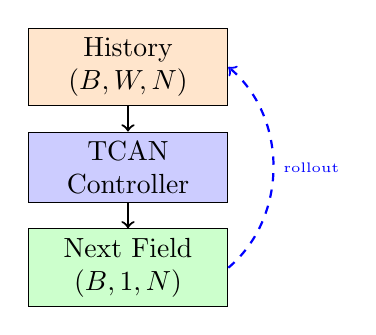
\begin{tikzpicture}[scale=0.75]

\node[rectangle, draw, fill=orange!20,
      text width=2.3cm, align=center,
      minimum height=0.65cm] 
(input) at (0, 2.8) {History\\$(B,W,N)$};

\node[rectangle, draw, fill=blue!20,
      text width=2.3cm, align=center,
      minimum height=0.65cm] 
(tcan) at (0, 1.1) {TCAN\\Controller};

\node[rectangle, draw, fill=green!20,
      text width=2.3cm, align=center,
      minimum height=0.65cm] 
(output) at (0, -0.6) {Next Field\\$(B,1,N)$};

\draw[->, thick] (input) -- (tcan);
\draw[->, thick] (tcan) -- (output);
\draw[->, thick, dashed, blue] (output.east)
      to[bend right=50] node[right, font=\tiny] {rollout} (input.east);

\end{tikzpicture}
\end{columns}
\end{frame}
